Podczas przygotowywania się do rozpoczęcia pracy z nową technologią, każdy
programista powinien być świadomy tego jakie są istniejące narzędzia, które mogą
mu pomóc w pracy. W tym rozdziale opisany jest sposób instalacji oraz używania
narzędzi wykorzystywanych przez autorów tej pracy.

\begin{figure}[!ht]
 \centering
 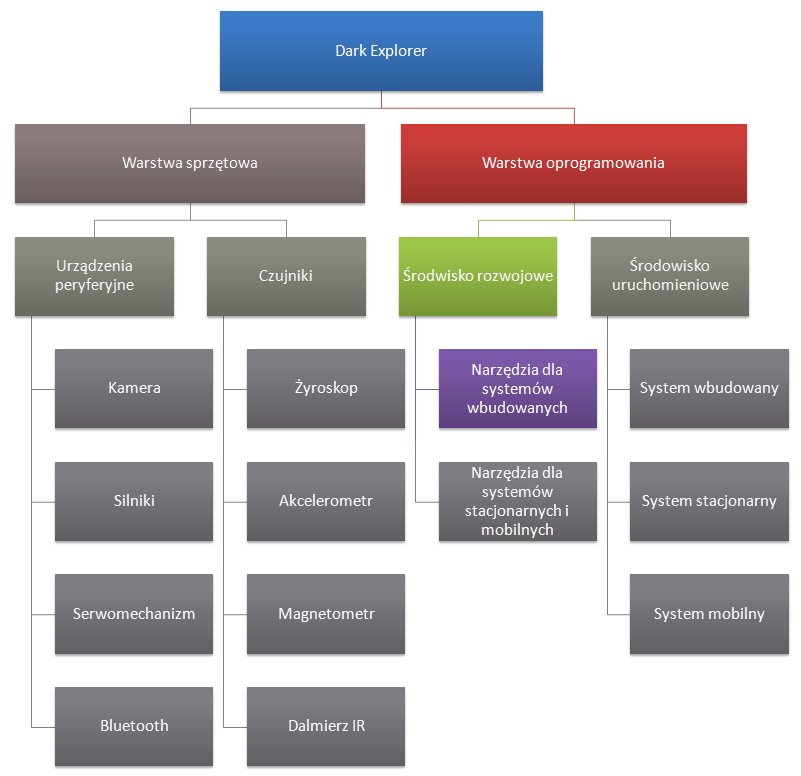
\includegraphics[height=125mm]{../images/ch03/dark_explorer_platform_ide_embeded.png}
 \caption{Struktura platformy robota mobilnego po zakończeniu prac. Kolorem oznaczono zakres prac opisanych w bierzącym rozdziale.}
 \label{fig:DarkExplorerPlatformIDE}
\end{figure}

\section{Narzędzia dla systemu Windows}
\label{sec:embeded-win-tools}
Pierwszym krokiem do przygotowania środowiska rozwojowego umożliwiającego
rozwijanie oprogramowania sterującego robotem jest instalacja sterowników
wymaganych przez system Windows do obsługi interfejsu JTAG\footnote{Joint Test
Action Group - jest to nazwa standardu który definuje protokół wykorzystywany do
testowania połączeń na płytkach drukowanych oraz uruchamiania i programowania
układów i systemów mikroprocesorowych. } za pomocą którego odbywa się proces
wgrywania przygotowanego oprogramowania do pamięci robota. Kolejnym wymaganym
krokiem jest instalacja i konfiguracja narzędzi umożliwiających stworzenie pliku
binarnego umożliwiającego uruchomienie przygotowanej na platformie sprzętowej
robota. Ostatnim etapem przygotowań jest instalacja oprogramowania
umożliwiającego programowanie układu za pomocą wspomnianego interfejsu JTAG oraz
debugowanie aplikacji w trakcie jej działania na robocie.

\subsection{Instalacja WinARM}
Do kompilacji kodu źródłowego oprogramowania zajmującego się sterowaniem
podzespołami robota wykorzystany został zestaw narzędzi znany pod nazwą WinARM.
WinARM jest zestawem narzędzi umożliwiających tworzenie oprogramowania dla
kontrolerów opartych na platformie ARM. W odróżnieniu od innych dostępnych
obecnie rozwiązań, środowisko to, nie wymaga dodatkowej instalacji narzędzi
udostępnianych w ramach MinGW\footnote{Minimalist GNU for Windows - port GCC
dostarczający zestaw darmowych narzędzi do komiplacji natywnych plików
wykonywalnych dla platformy Windows} czy też Cygwina\footnote{Cygwin -
implementacja standardu POSIX przeznaczona dla systemów z rodziny Windows}.
Wszystkie potrzebne narzędzia dostarczane są w ramach SDK\footnote{SDK (z ang.
Software Development Kit) - Zestaw narzędzi do rozwoju oprogramowania}. Narzędzia
WinARM pomyślnie przeszły testy z kontrolerami Atmel AT91SAM7S64, AT91SAM7S256,
AT91RM9200 ARM7TDMI oraz Philips LPC2106, Philips LPC2129, Philips LPC2138,
Philips LPC2148. Dodatkowo dostarczane w ramach środowiska kompilatory i
narzędzia powinny prawidłowo współpracować ze wszystkimi mikrokontrolerami
opartymi o architekturę ARM(-TDMI/Thumb itp.).

Instalację środowiska WinARM należy rozpocząć od pobrania archiwum z najnowszą
wersją narzędzi ze strony
\url{http://gandalf.arubi.uni-kl.de/avr_projects/arm_projects/}. W chwili pisania
pracy dostępna była wersja środowiska WinARM w wersji 20060606. Po zakończeniu
procesu pobierania, archiwum należy rozpakować w taki sposób aby wszystkie
podstawowe narzędzia dostępne były w katalogu \url{C:\WinARM\bin}. Umieszczenie
katalogu z narzędziami WinARM w innej lokalizacji jest również możliwe, ale może
wymagać wykonania dodatkowych operacji konfiguracyjnych w celu zapewnienia
poprawności działania wszystkich narzędzi. Aby udostępnić narzędzia WinARM z
linii poleceń systemu Windows konieczne jest dodanie do zmiennej systemowej
\url{PATH} ścieżki do katalogów z plikami wykonywalnymi biblioteki. W przypadku
instalacji w podanym powyżej katalogu wartości powinny być następujące
\url{C:\WinARM\bin;C:\WinARM\utils\bin;}. Jeżeli jednak katalog z pakietem
został umieszczony w innej lokalizacji konieczne jest odpowiednie zmodyfikowanie
wspomnianych wpisów. Szczegóły okna konfiguracji widoczne są na rysunku
\ref{fig:winarm-config}

\begin{figure}[h!]
 \centering
 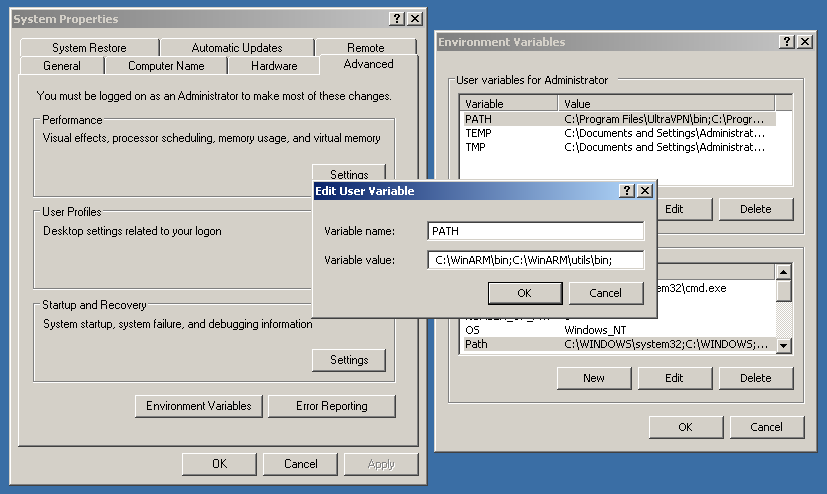
\includegraphics[width=0.95\textwidth]{../images/ch03/winarm-config-win32.png}
 \caption{Konfiguracja narzędzi pakietu WinARM}
 \label{fig:winarm-config}
\end{figure}

\subsection{Instalacja sterowników programatora}
Programowanie oraz debugowanie aplikacji robota może zostać zrealizowane za
pomocą dowolnego programatora kompatybilnego z interfejsem JTAG. Programatory
oparte o interfejs LPT nie wymagają od użytkownika żadnej dodatkowej
konfiguracji. Nieco inaczej wygląda sytuacja z programatorami opartymi o
interfejs USB, które to wymagają przed pierwszym użyciem zainstalowania
sterowników umożliwiających prawidłowe rozpoznanie programatora przez system
Windows. Jednym z bardziej popularnych programatorów USB jest TriTon JTAG. TriTon
JTAG to programator przeznaczony dla procesorów zbudowanych w oparciu o rdzeń ARM
podłączany do komputera za pomocą portu USB. TriTon JTAG posiada standardowe 20
pinowe złącze JTAG wraz z wyprowadzeniami sygnałów RxD i TxD interfejsu UART.
TriTon JTAG współpracuje z OpenOCD, pozwalając na programowanie oraz debugowanie
działającej na urządzeniu aplikacji. Urządzenie oparte jest o układ FT2232 który
umożliwia jego współprace także z innymi środowiskami rozwoju oprogramowania dla
platformy ARM kompatybilnymi z FT2232.

\begin{figure}[h!]
 \centering
 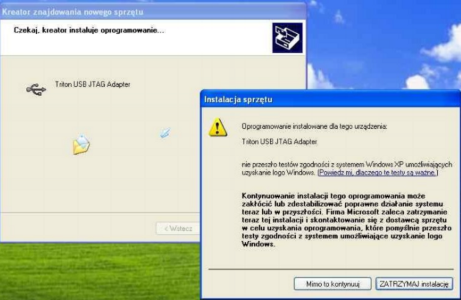
\includegraphics[width=0.85\textwidth]{../images/ch03/jtag-install-s2.png}
 \caption{Instalacja sterowników do programatora TriTon JTAG}
 \label{fig:TritonInstall}
\end{figure}

Instalację programatora należy rozpocząć od pobrania sterowników do układu FT2232
ze strony \url{http://www.ethernut.de/en/download/}. Na stronie dostępne są
sterowniki przeznaczone dla systemów Windows 2000, XP, Server 2003, Vista oraz
Server 2008. Po rozpakowaniu archiwum ze sterownikami należy za pomocą interfejsu
USB podłączyć programator do komputera. Po wykryciu system Windows trzykrotnie
poprosi o podanie ścieżki do sterowników do urządzeń Triton JTAG, Triton USB
RS232 Adapter oraz USB Serial Port. Należy wtedy skazać ścieżkę do katalogu w
którym rozpakowane zostały sterowniki pobrane ze strony wspomnianej wcześniej. Po
poprawnym zakończeniu instalacji w Menadżerze urządzeń systemu Windows widoczne
będą następujące elementy
\begin{itemize}
  \item Triton USB JTAG Adapter,
  \item Triton USB RS232 Adapter,
  \item Triton JTAG
\end{itemize}

\subsection{Instalacja Open On-Chip Debugger}
OpenOCD zostało zapoczątkowane przez Dominika Rath w ramach pracy dyplomowej
realizowanej na uniwersytecie w Augsburg. Od tamtego czasu OpenOCD bardzo się
rozwinęło i urosło do rozmiarów aktywnego projektu open-sourcowego wspieranego
przez programistów z całego świata. Celem OpenOCD jest dostarczenie
uniwersalnego narzędzia umożliwiającego debugowanie i programowanie systemów
wbudowanych.
 
\begin{figure}[h!]
 \centering
 \subfloat{\label{fig:OpenOCD-A}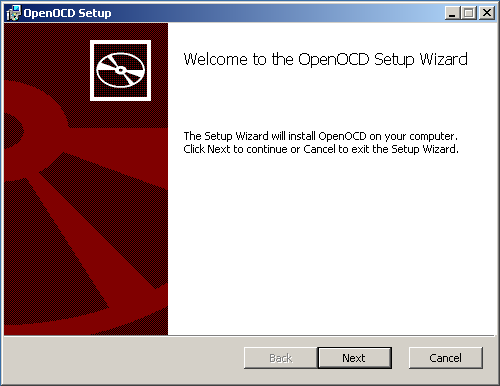
\includegraphics[width=0.7\textwidth]{../images/ch03/open-ocd-install-s1.png}}\hfill
 \subfloat{\label{fig:OpenOCD-B}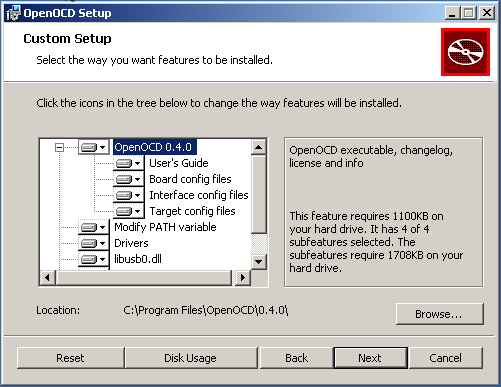
\includegraphics[width=0.7\textwidth]{../images/ch03/open-ocd-install-s2.png}}
 \caption{Instalator Open On-Chip Debugger'a (OpenOCD)}
 \label{fig:openocd-win32-install}
\end{figure}

Strona projektu OpenOCD dostępna jest pod adresem
\url{http://openocd.berlios.de/web/}. Dostępne są tam zarówno źródła jak i
dokumentacja do projektu. Niestety w chwili pisania pracy magisterskiej autorzy
nie udostępniali wersji skompilowanej dla systemu Windows. Dlatego też użyta
została niezależna wersja OpenOCD z przygotowanym instalatorem dla systemu
Windows. Instalator OpenOCD dla Windows jest do pobrania ze strony
\url{http://www.ethernut.de/en/download/}. Po uruchomieniu instalatora wybieramy
lokalizację docelową w której OpenOCD ma zostać zainstalowane. Po zakończeniu
instalacji konieczne jest uzupełnienie wartości zmiennej systemowej PATH ścieżką
do miejsca instalacji OpenOCD, domyślnie \url{C:\ethernut\nut\tools\win32}.

\subsection{Konfiguracja zintegrowanego środowiska programistycznego}
Poprawne zainstalowanie pakietów WinARM oraz OpenOCD dostarcza wszystkich
niezbędnych narzędzi potrzebnych do rozwijania aplikacji dla platform
wbudowanych. Niemniej jednak korzystanie z nich wymaga bezpośredniej interakcji
z linią poleceń systemu Windows, co dla niektórych programistów może być
uciążliwe. Możliwe jest napisanie skryptów systemowych pozwalających na
uruchamianie sekwencji procedur wymaganych np. do zaprogramowania robota,
ale jest to rozwiązanie nieprzenośne i słabo konfigurowalne. Dlatego też zaleca
się instalację zintegrowanego środowiska programistycznego które oprócz edytora
kodu umożliwi automatyzację najczęściej wykonywanych zadań. Wybór rodzaju
środowiska programistycznego zależy niemal w całości od preferencji programisty
gdyż większość potrzebnych narzędzi można bez większych trudności zintegrować z
ulubionym edytorem. Na potrzeby tej pracy omówiona zostanie konfiguracja dla
środowiska Eclipse. Wybór podyktowany został faktem iż jest to obecnie jedna z
najpopularniejszych platform do rozwoju oprogramowania, a co więcej jej
konfiguracja przebiega identycznie dla systemu Windows jak i Linux. Z tego
względu szczegółowy opis procedury konfiguracji zamieszczony został w rozdziale
poświęconym narzędziom dla systemu Linux.
